%!TEX root = ../ycac2vec.tex

\subsection{Plausibility of embedding space}

Word embedding models of natural language can be evaluated for their plausibility by comparing distances between points in the learned space and benchmark data. These data usually consist in taxonomies of semantically similar concepts established by usage or extracted from expert knowledge. 

In the musical case, there are is no established ways to evaluate embedding spaces trained on musical corpora. To establish the plausbility of our embedding space trained on the whole musical corpus, we query the space for the ten pitch-class sets that are closest to the set corresponding to the C major triad (Table \ref{tab:close_to_c}). We see that most of the ten closest chords can be analysed as having a root of C. In conventional tonal analysis we would likely consider these pitch-class sets as expressing some contrapuntal phenomena, such as suspensions and passing notes.

Since our corpus is trained on sequences of salami-sliced musical textures only, it is by design na\"{i}ve with respect to counterpoint. Nevertheless, the nearest neighbors to major triads are thos pitch-class sets which are often analyzed as expressions of the major triad that is nearest in voice-leading terms. We conclude that the model captures this intuition of tonal harmony but expect further work to develop the evaluation of embedding spaces with respect to benchmark data or other measures of harmonic similarity.  

\begin{table}

 \begin{center}
 \begin{tabular}{|l|l|l|}

  \hline
  Pitch-class set & Chord Symbol & Similarity  \\
\hline
\hline
$\langle C, D, E, G \rangle$ & CaddD & 0.65 \\
\hline
$\langle C, E, F, G \rangle$ & CaddF & 0.61 \\
\hline
$\langle C, E, G, B \rangle$ & Cmaj7 & 0.59 \\
\hline
$\langle C, D, E, F, G \rangle$ & CaddD,F & 0.56 \\
\hline
$\langle C, E, F\sharp, G \rangle$ & CaddF$\sharp$ & 0.55 \\
\hline
$\langle C, E\flat, E, F\sharp, G \rangle$ & Cmadd$\sharp$,E & 0.55 \\
\hline
$\langle C, E\flat, E, G \rangle$ & CmaddE & 0.52 \\
\hline
$\langle C, E, G, G\sharp \rangle$ & CaddG$\sharp$ & 0.48 \\
\hline
$\langle C, E, G, A \rangle$ & Am7/C & 0.48 \\
\hline
$\langle C, E \rangle$ & NC & 0.46 \\
\hline



\end{tabular}
\end{center}

 \caption{Ten closest chords to C major in the embedding space trained on the whole corpus}
 \label{tab:close_to_c}
\end{table}

\subsection{Analysis of time-delimited subcorpora}
Each time-delimited subcorpus was used to train a word embedding model. The model was parameterized to embedded the resulting spaces in $\mathbf{R}^{100}$, so we use principal component analysis (PCA) to visualize the structure of each space in the figures described below.

Figure \ref{fig:1700_majors} shows the locations of all twelve major triads in the embedding space trained on music from 1700--1749, as represented by the coefficients for the first two principal components. Arrows connect pairs of major triads such that arrows originate from the dominant of its target, in the key of represented by the target triad. For instance, since in the key of C major

$$\textrm{G major} \xrightarrow{\textrm{dominant of}} \textrm{C major}$$

the location in the space corresponding to the G major triad is joined with an arrow to that corresponding to the C major triad.  

We make the following qualitative observations:
\begin{enumerate}
\item The major triads are arranged in a circular topology
\item The order of major triads in this arrangement respects their order in the circle of fifths. That is, the roots of adjacent triads are related by the interval of a perfect fifth.
\end{enumerate}
In light of Figures \ref{fig:1750_majors}--\ref{fig:1850_majors}, which represent embedding spaces trained on music from later 50-year periods, we add:
\begin{enumerate}[resume]
\item The arrangement of major triads becomes more deformed as models trained on music from a later period are considered, while remaining topologically regular.
\end{enumerate}


\begin{figure}
 \centerline{\framebox{
 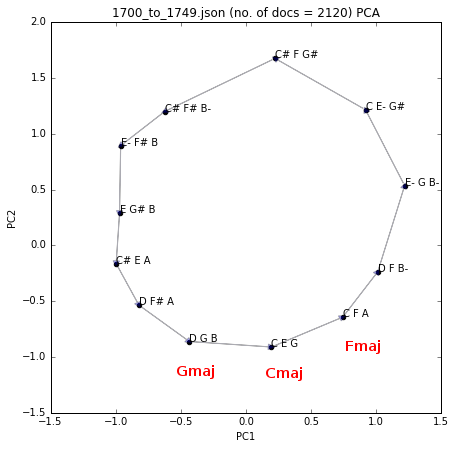
\includegraphics[width=\columnwidth]{figs/1700_majors.png}}}
 \caption{Coefficients for the first two principal components for major chords in PCA-reduced embedding space trained on pieces composed between 1700--1749.}
 \label{fig:1700_majors}
\end{figure}

\begin{figure}
 \centerline{\framebox{
 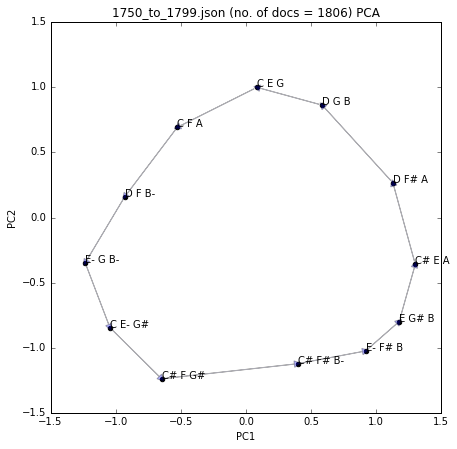
\includegraphics[width=\columnwidth]{figs/1750_majors.png}}}
 \caption{Coefficients for the first two principal components for major chords in PCA-reduced embedding space trained on pieces composed between 1750--1799.}
 \label{fig:1750_majors}
\end{figure}


\begin{figure}
 \centerline{\framebox{
 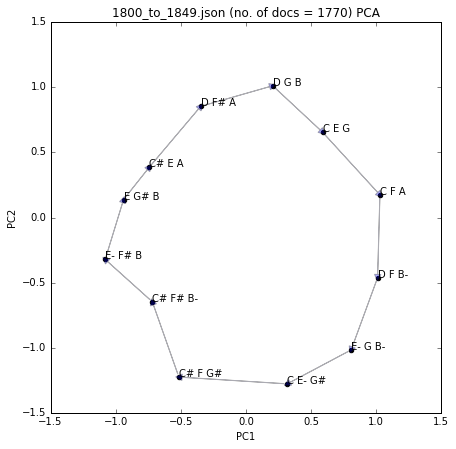
\includegraphics[width=\columnwidth]{figs/1800_majors.png}}}
 \caption{Coefficients for the first two principal components for major chords in PCA-reduced embedding space trained on pieces composed between 1800--1849.}
 \label{fig:1800_majors}
\end{figure}


\begin{figure}
 \centerline{\framebox{
 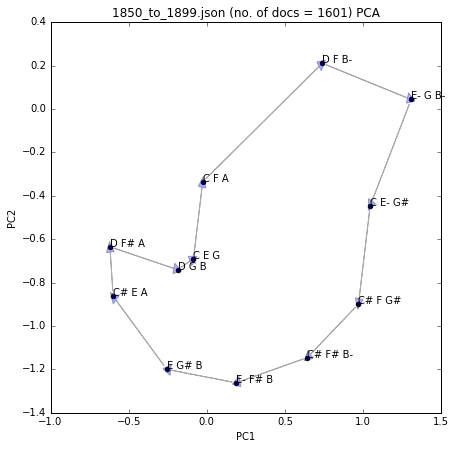
\includegraphics[width=\columnwidth]{figs/1850_majors.png}}}
 \caption{Coefficients for the first two principal components for major chords in PCA-reduced embedding space trained on pieces composed between 1850--1899.}
 \label{fig:1850_majors}
\end{figure}

